% Options for packages loaded elsewhere
\PassOptionsToPackage{unicode}{hyperref}
\PassOptionsToPackage{hyphens}{url}
\PassOptionsToPackage{dvipsnames,svgnames,x11names}{xcolor}
%
\documentclass[
  letterpaper,
]{report}

\usepackage{amsmath,amssymb}
\usepackage{iftex}
\ifPDFTeX
  \usepackage[T1]{fontenc}
  \usepackage[utf8]{inputenc}
  \usepackage{textcomp} % provide euro and other symbols
\else % if luatex or xetex
  \usepackage{unicode-math}
  \defaultfontfeatures{Scale=MatchLowercase}
  \defaultfontfeatures[\rmfamily]{Ligatures=TeX,Scale=1}
\fi
\usepackage{lmodern}
\ifPDFTeX\else  
    % xetex/luatex font selection
\fi
% Use upquote if available, for straight quotes in verbatim environments
\IfFileExists{upquote.sty}{\usepackage{upquote}}{}
\IfFileExists{microtype.sty}{% use microtype if available
  \usepackage[]{microtype}
  \UseMicrotypeSet[protrusion]{basicmath} % disable protrusion for tt fonts
}{}
\makeatletter
\@ifundefined{KOMAClassName}{% if non-KOMA class
  \IfFileExists{parskip.sty}{%
    \usepackage{parskip}
  }{% else
    \setlength{\parindent}{0pt}
    \setlength{\parskip}{6pt plus 2pt minus 1pt}}
}{% if KOMA class
  \KOMAoptions{parskip=half}}
\makeatother
\usepackage{xcolor}
\setlength{\emergencystretch}{3em} % prevent overfull lines
\setcounter{secnumdepth}{5}
% Make \paragraph and \subparagraph free-standing
\makeatletter
\ifx\paragraph\undefined\else
  \let\oldparagraph\paragraph
  \renewcommand{\paragraph}{
    \@ifstar
      \xxxParagraphStar
      \xxxParagraphNoStar
  }
  \newcommand{\xxxParagraphStar}[1]{\oldparagraph*{#1}\mbox{}}
  \newcommand{\xxxParagraphNoStar}[1]{\oldparagraph{#1}\mbox{}}
\fi
\ifx\subparagraph\undefined\else
  \let\oldsubparagraph\subparagraph
  \renewcommand{\subparagraph}{
    \@ifstar
      \xxxSubParagraphStar
      \xxxSubParagraphNoStar
  }
  \newcommand{\xxxSubParagraphStar}[1]{\oldsubparagraph*{#1}\mbox{}}
  \newcommand{\xxxSubParagraphNoStar}[1]{\oldsubparagraph{#1}\mbox{}}
\fi
\makeatother

\usepackage{color}
\usepackage{fancyvrb}
\newcommand{\VerbBar}{|}
\newcommand{\VERB}{\Verb[commandchars=\\\{\}]}
\DefineVerbatimEnvironment{Highlighting}{Verbatim}{commandchars=\\\{\}}
% Add ',fontsize=\small' for more characters per line
\usepackage{framed}
\definecolor{shadecolor}{RGB}{241,243,245}
\newenvironment{Shaded}{\begin{snugshade}}{\end{snugshade}}
\newcommand{\AlertTok}[1]{\textcolor[rgb]{0.68,0.00,0.00}{#1}}
\newcommand{\AnnotationTok}[1]{\textcolor[rgb]{0.37,0.37,0.37}{#1}}
\newcommand{\AttributeTok}[1]{\textcolor[rgb]{0.40,0.45,0.13}{#1}}
\newcommand{\BaseNTok}[1]{\textcolor[rgb]{0.68,0.00,0.00}{#1}}
\newcommand{\BuiltInTok}[1]{\textcolor[rgb]{0.00,0.23,0.31}{#1}}
\newcommand{\CharTok}[1]{\textcolor[rgb]{0.13,0.47,0.30}{#1}}
\newcommand{\CommentTok}[1]{\textcolor[rgb]{0.37,0.37,0.37}{#1}}
\newcommand{\CommentVarTok}[1]{\textcolor[rgb]{0.37,0.37,0.37}{\textit{#1}}}
\newcommand{\ConstantTok}[1]{\textcolor[rgb]{0.56,0.35,0.01}{#1}}
\newcommand{\ControlFlowTok}[1]{\textcolor[rgb]{0.00,0.23,0.31}{\textbf{#1}}}
\newcommand{\DataTypeTok}[1]{\textcolor[rgb]{0.68,0.00,0.00}{#1}}
\newcommand{\DecValTok}[1]{\textcolor[rgb]{0.68,0.00,0.00}{#1}}
\newcommand{\DocumentationTok}[1]{\textcolor[rgb]{0.37,0.37,0.37}{\textit{#1}}}
\newcommand{\ErrorTok}[1]{\textcolor[rgb]{0.68,0.00,0.00}{#1}}
\newcommand{\ExtensionTok}[1]{\textcolor[rgb]{0.00,0.23,0.31}{#1}}
\newcommand{\FloatTok}[1]{\textcolor[rgb]{0.68,0.00,0.00}{#1}}
\newcommand{\FunctionTok}[1]{\textcolor[rgb]{0.28,0.35,0.67}{#1}}
\newcommand{\ImportTok}[1]{\textcolor[rgb]{0.00,0.46,0.62}{#1}}
\newcommand{\InformationTok}[1]{\textcolor[rgb]{0.37,0.37,0.37}{#1}}
\newcommand{\KeywordTok}[1]{\textcolor[rgb]{0.00,0.23,0.31}{\textbf{#1}}}
\newcommand{\NormalTok}[1]{\textcolor[rgb]{0.00,0.23,0.31}{#1}}
\newcommand{\OperatorTok}[1]{\textcolor[rgb]{0.37,0.37,0.37}{#1}}
\newcommand{\OtherTok}[1]{\textcolor[rgb]{0.00,0.23,0.31}{#1}}
\newcommand{\PreprocessorTok}[1]{\textcolor[rgb]{0.68,0.00,0.00}{#1}}
\newcommand{\RegionMarkerTok}[1]{\textcolor[rgb]{0.00,0.23,0.31}{#1}}
\newcommand{\SpecialCharTok}[1]{\textcolor[rgb]{0.37,0.37,0.37}{#1}}
\newcommand{\SpecialStringTok}[1]{\textcolor[rgb]{0.13,0.47,0.30}{#1}}
\newcommand{\StringTok}[1]{\textcolor[rgb]{0.13,0.47,0.30}{#1}}
\newcommand{\VariableTok}[1]{\textcolor[rgb]{0.07,0.07,0.07}{#1}}
\newcommand{\VerbatimStringTok}[1]{\textcolor[rgb]{0.13,0.47,0.30}{#1}}
\newcommand{\WarningTok}[1]{\textcolor[rgb]{0.37,0.37,0.37}{\textit{#1}}}

\providecommand{\tightlist}{%
  \setlength{\itemsep}{0pt}\setlength{\parskip}{0pt}}\usepackage{longtable,booktabs,array}
\usepackage{calc} % for calculating minipage widths
% Correct order of tables after \paragraph or \subparagraph
\usepackage{etoolbox}
\makeatletter
\patchcmd\longtable{\par}{\if@noskipsec\mbox{}\fi\par}{}{}
\makeatother
% Allow footnotes in longtable head/foot
\IfFileExists{footnotehyper.sty}{\usepackage{footnotehyper}}{\usepackage{footnote}}
\makesavenoteenv{longtable}
\usepackage{graphicx}
\makeatletter
\newsavebox\pandoc@box
\newcommand*\pandocbounded[1]{% scales image to fit in text height/width
  \sbox\pandoc@box{#1}%
  \Gscale@div\@tempa{\textheight}{\dimexpr\ht\pandoc@box+\dp\pandoc@box\relax}%
  \Gscale@div\@tempb{\linewidth}{\wd\pandoc@box}%
  \ifdim\@tempb\p@<\@tempa\p@\let\@tempa\@tempb\fi% select the smaller of both
  \ifdim\@tempa\p@<\p@\scalebox{\@tempa}{\usebox\pandoc@box}%
  \else\usebox{\pandoc@box}%
  \fi%
}
% Set default figure placement to htbp
\def\fps@figure{htbp}
\makeatother
% definitions for citeproc citations
\NewDocumentCommand\citeproctext{}{}
\NewDocumentCommand\citeproc{mm}{%
  \begingroup\def\citeproctext{#2}\cite{#1}\endgroup}
\makeatletter
 % allow citations to break across lines
 \let\@cite@ofmt\@firstofone
 % avoid brackets around text for \cite:
 \def\@biblabel#1{}
 \def\@cite#1#2{{#1\if@tempswa , #2\fi}}
\makeatother
\newlength{\cslhangindent}
\setlength{\cslhangindent}{1.5em}
\newlength{\csllabelwidth}
\setlength{\csllabelwidth}{3em}
\newenvironment{CSLReferences}[2] % #1 hanging-indent, #2 entry-spacing
 {\begin{list}{}{%
  \setlength{\itemindent}{0pt}
  \setlength{\leftmargin}{0pt}
  \setlength{\parsep}{0pt}
  % turn on hanging indent if param 1 is 1
  \ifodd #1
   \setlength{\leftmargin}{\cslhangindent}
   \setlength{\itemindent}{-1\cslhangindent}
  \fi
  % set entry spacing
  \setlength{\itemsep}{#2\baselineskip}}}
 {\end{list}}
\usepackage{calc}
\newcommand{\CSLBlock}[1]{\hfill\break\parbox[t]{\linewidth}{\strut\ignorespaces#1\strut}}
\newcommand{\CSLLeftMargin}[1]{\parbox[t]{\csllabelwidth}{\strut#1\strut}}
\newcommand{\CSLRightInline}[1]{\parbox[t]{\linewidth - \csllabelwidth}{\strut#1\strut}}
\newcommand{\CSLIndent}[1]{\hspace{\cslhangindent}#1}

\makeatletter
\@ifpackageloaded{bookmark}{}{\usepackage{bookmark}}
\makeatother
\makeatletter
\@ifpackageloaded{caption}{}{\usepackage{caption}}
\AtBeginDocument{%
\ifdefined\contentsname
  \renewcommand*\contentsname{Table of contents}
\else
  \newcommand\contentsname{Table of contents}
\fi
\ifdefined\listfigurename
  \renewcommand*\listfigurename{List of Figures}
\else
  \newcommand\listfigurename{List of Figures}
\fi
\ifdefined\listtablename
  \renewcommand*\listtablename{List of Tables}
\else
  \newcommand\listtablename{List of Tables}
\fi
\ifdefined\figurename
  \renewcommand*\figurename{Figure}
\else
  \newcommand\figurename{Figure}
\fi
\ifdefined\tablename
  \renewcommand*\tablename{Table}
\else
  \newcommand\tablename{Table}
\fi
}
\@ifpackageloaded{float}{}{\usepackage{float}}
\floatstyle{ruled}
\@ifundefined{c@chapter}{\newfloat{codelisting}{h}{lop}}{\newfloat{codelisting}{h}{lop}[chapter]}
\floatname{codelisting}{Listing}
\newcommand*\listoflistings{\listof{codelisting}{List of Listings}}
\makeatother
\makeatletter
\makeatother
\makeatletter
\@ifpackageloaded{caption}{}{\usepackage{caption}}
\@ifpackageloaded{subcaption}{}{\usepackage{subcaption}}
\makeatother
\makeatletter
\@ifpackageloaded{sidenotes}{}{\usepackage{sidenotes}}
\@ifpackageloaded{marginnote}{}{\usepackage{marginnote}}
\makeatother

\usepackage{bookmark}

\IfFileExists{xurl.sty}{\usepackage{xurl}}{} % add URL line breaks if available
\urlstyle{same} % disable monospaced font for URLs
\hypersetup{
  pdftitle={Advanced Neuroimaging},
  pdfauthor={Natalia Zaretskaya},
  colorlinks=true,
  linkcolor={blue},
  filecolor={Maroon},
  citecolor={Blue},
  urlcolor={Blue},
  pdfcreator={LaTeX via pandoc}}


\title{Advanced Neuroimaging}
\usepackage{etoolbox}
\makeatletter
\providecommand{\subtitle}[1]{% add subtitle to \maketitle
  \apptocmd{\@title}{\par {\large #1 \par}}{}{}
}
\makeatother
\subtitle{PSY.842}
\author{Natalia Zaretskaya}
\date{SS 2025}

\begin{document}
\maketitle

\renewcommand*\contentsname{Table of contents}
{
\hypersetup{linkcolor=}
\setcounter{tocdepth}{2}
\tableofcontents
}

\bookmarksetup{startatroot}

\chapter*{Welcome!}\label{welcome}
\addcontentsline{toc}{chapter}{Welcome!}

\markboth{Welcome!}{Welcome!}

\includegraphics[width=1.04167in,height=\textheight,keepaspectratio]{images/claus_7TCOR_activity_website.png}

\begin{longtable}[]{@{}
  >{\raggedright\arraybackslash}p{(\linewidth - 8\tabcolsep) * \real{0.1000}}
  >{\raggedright\arraybackslash}p{(\linewidth - 8\tabcolsep) * \real{0.2000}}
  >{\raggedright\arraybackslash}p{(\linewidth - 8\tabcolsep) * \real{0.3000}}
  >{\raggedright\arraybackslash}p{(\linewidth - 8\tabcolsep) * \real{0.3000}}
  >{\raggedright\arraybackslash}p{(\linewidth - 8\tabcolsep) * \real{0.1000}}@{}}
\caption{Course schedule}\label{tbl-schedule}\tabularnewline
\toprule\noalign{}
\endfirsthead
\endhead
\bottomrule\noalign{}
\endlastfoot
\begin{minipage}[t]{\linewidth}\raggedright
\bookmarksetup{startatroot}

\chapter*{Session \#}\label{session}
\addcontentsline{toc}{chapter}{Session \#}

\markboth{Session \#}{Session \#}
\end{minipage} & \begin{minipage}[t]{\linewidth}\raggedright
\bookmarksetup{startatroot}

\chapter*{Date and time}\label{date-and-time}
\addcontentsline{toc}{chapter}{Date and time}

\markboth{Date and time}{Date and time}
\end{minipage} & \begin{minipage}[t]{\linewidth}\raggedright
\bookmarksetup{startatroot}

\chapter*{Specific topic}\label{specific-topic}
\addcontentsline{toc}{chapter}{Specific topic}

\markboth{Specific topic}{Specific topic}
\end{minipage} & \begin{minipage}[t]{\linewidth}\raggedright
\bookmarksetup{startatroot}

\chapter*{TODO for this class}\label{todo-for-this-class}
\addcontentsline{toc}{chapter}{TODO for this class}

\markboth{TODO for this class}{TODO for this class}
\end{minipage} & \begin{minipage}[t]{\linewidth}\raggedright
\bookmarksetup{startatroot}

\chapter*{Estimated workload (h)}\label{estimated-workload-h}
\addcontentsline{toc}{chapter}{Estimated workload (h)}

\markboth{Estimated workload (h)}{Estimated workload (h)}
\end{minipage} \\
\textbf{1} &
\href{https://online.uni-graz.at/kfu_online/pl/ui/$ctx/!wbTermin.wbEdit?pTerminNr=8700320}{\textbf{04.03.2025}}
\textbf{\textbar{} 13:30 \textbar{}
\href{https://online.uni-graz.at/kfu_online/pl/ui/$ctx/wbKalender.wbRessource?pResNr=12603&pDatum=04.03.2025&pOrgNr=&pSachbearbeiter=F}{SR
02.31 (0002030122)}} & \textbf{Organization and introduction} &
\textbf{none} & \textbf{0} \\
\textbf{2} &
\href{https://online.uni-graz.at/kfu_online/pl/ui/$ctx/!wbTermin.wbEdit?pTerminNr=8700319}{\textbf{11.03.2025}}
\textbf{\textbar{} 13:30 \textbar{}
\href{https://online.uni-graz.at/kfu_online/pl/ui/$ctx/wbKalender.wbRessource?pResNr=12603&pDatum=11.03.2025&pOrgNr=&pSachbearbeiter=F}{SR
02.31 (0002030122)}} & \href{fmri-intro.qmd}{\textbf{Introduction to
fMRI}} & \textbf{Make groups, start thinking of a project};

\textbf{Install PsychoPy} & 4 \\
\textbf{3} &
\href{https://online.uni-graz.at/kfu_online/pl/ui/$ctx/!wbTermin.wbEdit?pTerminNr=8700318}{\textbf{18.03.2025}}
\textbf{\textbar{} 13:30 \textbar{}
\href{https://online.uni-graz.at/kfu_online/pl/ui/$ctx/wbKalender.wbRessource?pResNr=12603&pDatum=18.03.2025&pOrgNr=&pSachbearbeiter=F}{SR
02.31 (0002030122)}} & \textbf{Project slam and public vote}

\textbf{(Winner does not need to write an interoduction)} &
\textbf{Prepare a presentation of your project (See
\hyperref[sec-presentation-guidelines]{Presentation Guidelines} and
\hyperref[sec-presentation-evaluation]{Presentation Evaluation
Criteria})} & \textbf{4} \\
\textbf{4} &
\href{https://online.uni-graz.at/kfu_online/pl/ui/$ctx/!wbTermin.wbEdit?pTerminNr=8700317}{\textbf{25.03.2025}}
\textbf{\textbar{} 13:30 \textbar{}
\href{https://online.uni-graz.at/kfu_online/pl/ui/$ctx/wbKalender.wbRessource?pResNr=12603&pDatum=25.03.2025&pOrgNr=&pSachbearbeiter=F}{SR
02.31 (0002030122)}} & \textbf{Implementation slam and second public
vote}

\textbf{(Winner does not need to write the experiment description)} &
\textbf{Go through the
\href{https://www.youtube.com/watch?v=GSv60zgQlB8}{PsychoPy intro}.}

\textbf{Implement your project in PsychoPy, show it to the class} &
\textbf{8} \\
\textbf{5} &
\href{https://online.uni-graz.at/kfu_online/pl/ui/$ctx/!wbTermin.wbEdit?pTerminNr=8700316}{\textbf{01.04.2025}}
\textbf{\textbar{} 13:30 \textbar{}
\href{https://online.uni-graz.at/kfu_online/pl/ui/$ctx/wbKalender.wbRessource?pResNr=12603&pDatum=01.04.2025&pOrgNr=&pSachbearbeiter=F}{SR
02.31 (0002030122)}} & \textbf{Data management I} & \textbf{Neurodesk
registration} & \textbf{4} \\
\textbf{6} &
\href{https://online.uni-graz.at/kfu_online/pl/ui/$ctx/!wbTermin.wbEdit?pTerminNr=8700315}{\textbf{08.04.2025}}
\textbf{\textbar{} 13:30 \textbar{}
\href{https://online.uni-graz.at/kfu_online/pl/ui/$ctx/wbKalender.wbRessource?pResNr=12603&pDatum=08.04.2025&pOrgNr=&pSachbearbeiter=F}{SR
02.31 (0002030122)}} & \textbf{Experiment feedback, data management II;}

\textbf{Data acquisition in the MRI lab 9.04.2025} & \textbf{Every
course participant performs 3 rounds of the experiment and gives
feedback} & \textbf{1} \\
7 &
\href{https://online.uni-graz.at/kfu_online/pl/ui/$ctx/!wbTermin.wbEdit?pTerminNr=8700314}{29.04.2025}
\textbar{} 13:30 \textbar{}
\href{https://online.uni-graz.at/kfu_online/pl/ui/$ctx/wbKalender.wbRessource?pResNr=12603&pDatum=29.04.2025&pOrgNr=&pSachbearbeiter=F}{SR
02.31 (0002030122)} & Preprocessing & MRIQC & 0 \\
8 &
\href{https://online.uni-graz.at/kfu_online/pl/ui/$ctx/!wbTermin.wbEdit?pTerminNr=8700313}{06.05.2025}
\textbar{} 13:30 \textbar{}
\href{https://online.uni-graz.at/kfu_online/pl/ui/$ctx/wbKalender.wbRessource?pResNr=12603&pDatum=06.05.2025&pOrgNr=&pSachbearbeiter=F}{SR
02.31 (0002030122)} & Analysis: General linear model & Preprocessing &
4 \\
9 &
\href{https://online.uni-graz.at/kfu_online/pl/ui/$ctx/!wbTermin.wbEdit?pTerminNr=8700312}{13.05.2025}
\textbar{} 13:30 \textbar{}
\href{https://online.uni-graz.at/kfu_online/pl/ui/$ctx/wbKalender.wbRessource?pResNr=12603&pDatum=13.05.2025&pOrgNr=&pSachbearbeiter=F}{SR
02.31 (0002030122)} & Analysis: Other analyses types & Data analysis &
4 \\
10 &
\href{https://online.uni-graz.at/kfu_online/pl/ui/$ctx/!wbTermin.wbEdit?pTerminNr=8700311}{20.05.2025}
\textbar{} 13:30 \textbar{}
\href{https://online.uni-graz.at/kfu_online/pl/ui/$ctx/wbKalender.wbRessource?pResNr=12603&pDatum=20.05.2025&pOrgNr=&pSachbearbeiter=F}{SR
02.31 (0002030122)} & Result visualization and reporting & Finish data
analysis & 4 \\
11 &
\href{https://online.uni-graz.at/kfu_online/pl/ui/$ctx/!wbTermin.wbEdit?pTerminNr=8700310}{27.05.2025}
\textbar{} 13:30 \textbar{}
\href{https://online.uni-graz.at/kfu_online/pl/ui/$ctx/wbKalender.wbRessource?pResNr=12603&pDatum=27.05.2025&pOrgNr=&pSachbearbeiter=F}{SR
02.31 (0002030122)} & Result presentation slam, public vote

(winner does not need to write a results section) & Prepare a poster
with images & 4 \\
12 &
\href{https://online.uni-graz.at/kfu_online/pl/ui/$ctx/!wbTermin.wbEdit?pTerminNr=8700309}{03.06.2025}
\textbar{} 13:30 \textbar{}
\href{https://online.uni-graz.at/kfu_online/pl/ui/$ctx/wbKalender.wbRessource?pResNr=12603&pDatum=03.06.2025&pOrgNr=&pSachbearbeiter=F}{SR
02.31 (0002030122)} & Writing an fMRI article & Report draft: Results
section & 4 \\
13 &
\href{https://online.uni-graz.at/kfu_online/pl/ui/$ctx/!wbTermin.wbEdit?pTerminNr=8700308}{17.06.2025}
\textbar{} 13:30 \textbar{}
\href{https://online.uni-graz.at/kfu_online/pl/ui/$ctx/wbKalender.wbRessource?pResNr=12603&pDatum=17.06.2025&pOrgNr=&pSachbearbeiter=F}{SR
02.31 (0002030122)} & Final session, course evaluation & Report draft &
4 \\
14 &
\href{https://online.uni-graz.at/kfu_online/pl/ui/$ctx/!wbTermin.wbEdit?pTerminNr=8700307}{24.06.2025}
\textbar{} 13:30 \textbar{}
\href{https://online.uni-graz.at/kfu_online/pl/ui/$ctx/wbKalender.wbRessource?pResNr=12603&pDatum=24.06.2025&pOrgNr=&pSachbearbeiter=F}{SR
02.31 (0002030122)} & Report deadline & & 4 \\
\end{longtable}

\bookmarksetup{startatroot}

\chapter*{Course Syllabus}\label{course-syllabus}
\addcontentsline{toc}{chapter}{Course Syllabus}

\markboth{Course Syllabus}{Course Syllabus}

\includegraphics[width=4.16667in,height=\textheight,keepaspectratio]{images/claus_7TCOR_activity_website.png}

Citation from UGOnline:

\emph{This practice-oriented seminar provides an introduction into the
modern methods of MRI-based neuroimaging for cognitive neuroscience.\\
It will take students through all stages of a functional MRI study:\\
- planning and programming an experiment,\\
- acquiring the data\\
- data preprocessing\\
- data analysis and interpretation\\
In addition to theoretical input, the course will have a strong
practical component. Students will first present their project ideas in
class. After this, the class will select the best project, which will be
implemented into a computer program. Together with the lecturer we will
conduct an fMRI experiment with one volunteer. The students will get
access to a server, and each person will go through all stages of data
preprocessing and analysis.\\
Open science practices in the field of neuroimaging will also be
introduced.}

\section*{Lecturer}\label{lecturer}
\addcontentsline{toc}{section}{Lecturer}

\markright{Lecturer}

Natalia Zaretskaya

Group Leader of the \href{https://neurovision.uni-graz.at/en/}{``Visual
Neuroscience Lab''}

\includegraphics[width=4.21875in,height=\textheight,keepaspectratio]{images/clipboard-890498128.png}

\section*{Contact information}\label{contact-information}
\addcontentsline{toc}{section}{Contact information}

\markright{Contact information}

\begin{itemize}
\tightlist
\item
  \href{mailto:natalia.zaretskaya@uni-graz.at}{\nolinkurl{natalia.zaretskaya@uni-graz.at}}
\item
  Office hours: Tuesdays 10:00-11:30, sign up via
  \url{https://doodle.com/bp/nataliazaretskaya/book-a-time}
\item
  Talk informally after class
\end{itemize}

\section*{Other courses}\label{other-courses}
\addcontentsline{toc}{section}{Other courses}

\markright{Other courses}

SS 2025

\begin{itemize}
\tightlist
\item
  BSc SE ``Neural Mechanisms of Consciousness''
\item
  MSc SE ``Advanced Neuroimaging Methods''
\end{itemize}

WS 2025

\begin{itemize}
\item
  BSc VL ``General Psychology I: Perception and Attention''
\item
  BSc KS ``Selected Studies in General Psychology''
\end{itemize}

\section*{Research interests}\label{research-interests}
\addcontentsline{toc}{section}{Research interests}

\markright{Research interests}

\begin{figure}[H]

{\centering \pandocbounded{\includegraphics[keepaspectratio]{images/clipboard-1154889361.png}}

}

\caption{For details, see
\url{https://neurovision.uni-graz.at/en/research-directions/}}

\end{figure}%

\section*{Organisatory aspects}\label{organisatory-aspects}
\addcontentsline{toc}{section}{Organisatory aspects}

\markright{Organisatory aspects}

\begin{itemize}
\item
  Let's be ``per du'' (Natalia)
\item
  Course language is English, but I speak German
\item
  Let's be less formal (please interrupt and ask questions!)
\item
  Course materials on Moodle: \url{https://moodle.uni-graz.at}
\end{itemize}

\section*{Content of the course}\label{content-of-the-course}
\addcontentsline{toc}{section}{Content of the course}

\markright{Content of the course}

\subsection*{``Hard'' knowledge}\label{hard-knowledge}
\addcontentsline{toc}{subsection}{``Hard'' knowledge}

\begin{itemize}
\tightlist
\item
  Basics of performing an fMRI experiment
\item
  Modern practices in fMRI data analysis
\item
  Open science practices in Neuroimaging
\end{itemize}

\subsection*{``Soft'' skills}\label{soft-skills}
\addcontentsline{toc}{subsection}{``Soft'' skills}

\begin{itemize}
\tightlist
\item
  Scientific presentations
\item
  Scientific writing
\item
  Critical thinking
\end{itemize}

\section*{Goals}\label{goals}
\addcontentsline{toc}{section}{Goals}

\markright{Goals}

\begin{itemize}
\item
  Understand the possibilities and limitations of functional MRI
\item
  Be able to plan, conduct, analyze and interpret fMRI experiments in
  practice
\item
  Know and apply open science practices in the field of neuroimaging
\end{itemize}

\section*{Possible workload for 4
ECTS}\label{possible-workload-for-4-ects}
\addcontentsline{toc}{section}{Possible workload for 4 ECTS}

\markright{Possible workload for 4 ECTS}

\begin{longtable}[]{@{}
  >{\raggedright\arraybackslash}p{(\linewidth - 6\tabcolsep) * \real{0.2500}}
  >{\raggedright\arraybackslash}p{(\linewidth - 6\tabcolsep) * \real{0.2500}}
  >{\raggedright\arraybackslash}p{(\linewidth - 6\tabcolsep) * \real{0.2500}}
  >{\raggedright\arraybackslash}p{(\linewidth - 6\tabcolsep) * \real{0.2500}}@{}}
\caption{Example workload distribution according to 4 ECTS (100
hours)}\label{tbl-ects}\tabularnewline
\toprule\noalign{}
\begin{minipage}[b]{\linewidth}\raggedright
\textbf{Activity}
\end{minipage} & \begin{minipage}[b]{\linewidth}\raggedright
\textbf{Hours per week}
\end{minipage} & \begin{minipage}[b]{\linewidth}\raggedright
\textbf{Total hours}
\end{minipage} & \begin{minipage}[b]{\linewidth}\raggedright
\textbf{Cumulative sum}
\end{minipage} \\
\midrule\noalign{}
\endfirsthead
\toprule\noalign{}
\begin{minipage}[b]{\linewidth}\raggedright
\textbf{Activity}
\end{minipage} & \begin{minipage}[b]{\linewidth}\raggedright
\textbf{Hours per week}
\end{minipage} & \begin{minipage}[b]{\linewidth}\raggedright
\textbf{Total hours}
\end{minipage} & \begin{minipage}[b]{\linewidth}\raggedright
\textbf{Cumulative sum}
\end{minipage} \\
\midrule\noalign{}
\endhead
\bottomrule\noalign{}
\endlastfoot
Classroom & 14 x 1.5 hours & 21 & 21 \\
Individual/group work & 14 x 4 & 56 & 77 \\
Report writing & & 23 hours ⁓ 3 full work days! & 100 \\
\textbf{Total} & & 100 & \\
\end{longtable}

\section*{Course requirements}\label{course-requirements}
\addcontentsline{toc}{section}{Course requirements}

\markright{Course requirements}

\begin{itemize}
\item
  Active participation in class (not graded)

  \begin{itemize}
  \item
    Attendance (maximum 2 absences are tolerated)
  \item
    Contribution to class work/discussions
  \item
    Homework submissions (see the \hyperref[tbl-schedule]{Course
    Schedule Table})
  \end{itemize}
\item
  25\%: Project concept presentation (individual or group)
\item
  25\%: Result visualization presentation (individual or group)
\item
  50 \%: Final report (individual)

  \begin{itemize}
  \tightlist
  \item
    After the deadline the grade decreases by 1 point per 24 hours
  \end{itemize}
\item
  Course feedback confirmation

  \begin{itemize}
  \tightlist
  \item
    Submission of an \href{https://online.uni-graz.at}{UGOnline}
    screenshot to \href{https://moodle.uni-graz.at}{Moodle} before
    semester end
  \end{itemize}
\end{itemize}

\section*{Evaluation criteria}\label{sec-presentation-evaluation}
\addcontentsline{toc}{section}{Evaluation criteria}

\markright{Evaluation criteria}

\begin{itemize}
\item
  Project presentation

  \begin{itemize}
  \item
    Scientific merit
  \item
    Feasibility
  \end{itemize}
\item
  Visualization presentation

  \begin{itemize}
  \tightlist
  \item
    Clarity in conveying the message
  \item
    Scientific correctness
  \end{itemize}
\item
  Report

  \begin{itemize}
  \item
    Formal correctness (see guidelines below)
  \item
    Understanding of all stages of course work
  \end{itemize}
\end{itemize}

\section*{Presentation guidelines}\label{sec-presentation-guidelines}
\addcontentsline{toc}{section}{Presentation guidelines}

\markright{Presentation guidelines}

\includegraphics[width=3.125in,height=\textheight,keepaspectratio]{images/classroom-1297780_1280.png}

\begin{itemize}
\item
  Duration 5-10 minutes
\item
  Aspects to address

  \begin{itemize}
  \item
    General relevance of the topic
  \item
    1-2 articles on the topic
  \item
    Specific research question
  \item
    Why is fMRI necessary?
  \item
    Specific experimental conditions\ldots?
  \end{itemize}
\end{itemize}

\section*{Report guidelines}\label{report-guidelines}
\addcontentsline{toc}{section}{Report guidelines}

\markright{Report guidelines}

\includegraphics[width=3.125in,height=\textheight,keepaspectratio]{images/classroom-1297781_1280.png}

\begin{itemize}
\item
  Introduction: maximum 500 words
\item
  Methods: max 1000 words

  \begin{itemize}
  \item
    Participant
  \item
    Experimental paradigm
  \item
    Data acquisition
  \item
    Data analysis
  \end{itemize}
\item
  Results: maximum 500 words
\item
  Discussion: maximum 500 words
\item
  References
\end{itemize}

\section*{AI usage (official)}\label{sec-ai-uni}
\addcontentsline{toc}{section}{AI usage (official)}

\markright{AI usage (official)}

\emph{The use of generative AI is generally possible in this course.
Please note, however, that you as a student bear full responsibility for
the accuracy of the generated content.}

\emph{An academic integrity statement is required for each submitted
paper, the verbatim copying of AI-generated text passages must be marked
- analogous to conventional citations - by stating the AI system and the
specification of the interaction (see
``\href{https://static.uni-graz.at/fileadmin/_files/_project_sites/_digitalelehre/Orientierungsrahmen/KI-Orientierungsrahmen_230901.pdf}{Orientation
guidelines for dealing with text-generating AI systems at the University
of Graz}'', p.~1-2).}

\emph{It is only prohibited to submit work that was created
predominantly or even exclusively using generative AI.}

\emph{When using generative AI, please ensure that your submissions do
not violate the rights of third parties, including copyright, personal
rights, and data protection regulations.}

\section*{AI usage (this course)}\label{sec-ai-course}
\addcontentsline{toc}{section}{AI usage (this course)}

\markright{AI usage (this course)}

AI usage is conditional on full disclosure:

\begin{itemize}
\item
  250 words maximum attachment to the report with a description of which
  AI tools were used and how exactly were they applied
\item
  You bare responsibility for the correctness and authorship of the
  written text
\item
  I keep the right to invite you and ask questions about the content
\end{itemize}

\section*{Course schedule}\label{course-schedule}
\addcontentsline{toc}{section}{Course schedule}

\markright{Course schedule}

\begin{longtable}[]{@{}
  >{\raggedright\arraybackslash}p{(\linewidth - 8\tabcolsep) * \real{0.1000}}
  >{\raggedright\arraybackslash}p{(\linewidth - 8\tabcolsep) * \real{0.2000}}
  >{\raggedright\arraybackslash}p{(\linewidth - 8\tabcolsep) * \real{0.3000}}
  >{\raggedright\arraybackslash}p{(\linewidth - 8\tabcolsep) * \real{0.3000}}
  >{\raggedright\arraybackslash}p{(\linewidth - 8\tabcolsep) * \real{0.1000}}@{}}
\caption{Course schedule}\label{tbl-schedule}\tabularnewline
\toprule\noalign{}
\endfirsthead
\endhead
\bottomrule\noalign{}
\endlastfoot
\begin{minipage}[t]{\linewidth}\raggedright
\bookmarksetup{startatroot}

\chapter*{Session \#}\label{session-1}
\addcontentsline{toc}{chapter}{Session \#}

\markboth{Session \#}{Session \#}
\end{minipage} & \begin{minipage}[t]{\linewidth}\raggedright
\bookmarksetup{startatroot}

\chapter*{Date and time}\label{date-and-time-1}
\addcontentsline{toc}{chapter}{Date and time}

\markboth{Date and time}{Date and time}
\end{minipage} & \begin{minipage}[t]{\linewidth}\raggedright
\bookmarksetup{startatroot}

\chapter*{Specific topic}\label{specific-topic-1}
\addcontentsline{toc}{chapter}{Specific topic}

\markboth{Specific topic}{Specific topic}
\end{minipage} & \begin{minipage}[t]{\linewidth}\raggedright
\bookmarksetup{startatroot}

\chapter*{TODO for this class}\label{todo-for-this-class-1}
\addcontentsline{toc}{chapter}{TODO for this class}

\markboth{TODO for this class}{TODO for this class}
\end{minipage} & \begin{minipage}[t]{\linewidth}\raggedright
\bookmarksetup{startatroot}

\chapter*{Estimated workload (h)}\label{estimated-workload-h-1}
\addcontentsline{toc}{chapter}{Estimated workload (h)}

\markboth{Estimated workload (h)}{Estimated workload (h)}
\end{minipage} \\
\textbf{1} &
\href{https://online.uni-graz.at/kfu_online/pl/ui/$ctx/!wbTermin.wbEdit?pTerminNr=8700320}{\textbf{04.03.2025}}
\textbf{\textbar{} 13:30 \textbar{}
\href{https://online.uni-graz.at/kfu_online/pl/ui/$ctx/wbKalender.wbRessource?pResNr=12603&pDatum=04.03.2025&pOrgNr=&pSachbearbeiter=F}{SR
02.31 (0002030122)}} & \textbf{Organization and introduction} &
\textbf{none} & \textbf{0} \\
\textbf{2} &
\href{https://online.uni-graz.at/kfu_online/pl/ui/$ctx/!wbTermin.wbEdit?pTerminNr=8700319}{\textbf{11.03.2025}}
\textbf{\textbar{} 13:30 \textbar{}
\href{https://online.uni-graz.at/kfu_online/pl/ui/$ctx/wbKalender.wbRessource?pResNr=12603&pDatum=11.03.2025&pOrgNr=&pSachbearbeiter=F}{SR
02.31 (0002030122)}} & \href{fmri-intro.qmd}{\textbf{Introduction to
fMRI}} & \textbf{Make groups, start thinking of a project};

\textbf{Install PsychoPy} & 4 \\
\textbf{3} &
\href{https://online.uni-graz.at/kfu_online/pl/ui/$ctx/!wbTermin.wbEdit?pTerminNr=8700318}{\textbf{18.03.2025}}
\textbf{\textbar{} 13:30 \textbar{}
\href{https://online.uni-graz.at/kfu_online/pl/ui/$ctx/wbKalender.wbRessource?pResNr=12603&pDatum=18.03.2025&pOrgNr=&pSachbearbeiter=F}{SR
02.31 (0002030122)}} & \textbf{Project slam and public vote}

\textbf{(Winner does not need to write an interoduction)} &
\textbf{Prepare a presentation of your project (See
\hyperref[sec-presentation-guidelines]{Presentation Guidelines} and
\hyperref[sec-presentation-evaluation]{Presentation Evaluation
Criteria})} & \textbf{4} \\
\textbf{4} &
\href{https://online.uni-graz.at/kfu_online/pl/ui/$ctx/!wbTermin.wbEdit?pTerminNr=8700317}{\textbf{25.03.2025}}
\textbf{\textbar{} 13:30 \textbar{}
\href{https://online.uni-graz.at/kfu_online/pl/ui/$ctx/wbKalender.wbRessource?pResNr=12603&pDatum=25.03.2025&pOrgNr=&pSachbearbeiter=F}{SR
02.31 (0002030122)}} & \textbf{Implementation slam and second public
vote}

\textbf{(Winner does not need to write the experiment description)} &
\textbf{Go through the
\href{https://www.youtube.com/watch?v=GSv60zgQlB8}{PsychoPy intro}.}

\textbf{Implement your project in PsychoPy, show it to the class} &
\textbf{8} \\
\textbf{5} &
\href{https://online.uni-graz.at/kfu_online/pl/ui/$ctx/!wbTermin.wbEdit?pTerminNr=8700316}{\textbf{01.04.2025}}
\textbf{\textbar{} 13:30 \textbar{}
\href{https://online.uni-graz.at/kfu_online/pl/ui/$ctx/wbKalender.wbRessource?pResNr=12603&pDatum=01.04.2025&pOrgNr=&pSachbearbeiter=F}{SR
02.31 (0002030122)}} & \textbf{Data management I} & \textbf{Neurodesk
registration} & \textbf{4} \\
\textbf{6} &
\href{https://online.uni-graz.at/kfu_online/pl/ui/$ctx/!wbTermin.wbEdit?pTerminNr=8700315}{\textbf{08.04.2025}}
\textbf{\textbar{} 13:30 \textbar{}
\href{https://online.uni-graz.at/kfu_online/pl/ui/$ctx/wbKalender.wbRessource?pResNr=12603&pDatum=08.04.2025&pOrgNr=&pSachbearbeiter=F}{SR
02.31 (0002030122)}} & \textbf{Experiment feedback, data management II;}

\textbf{Data acquisition in the MRI lab 9.04.2025} & \textbf{Every
course participant performs 3 rounds of the experiment and gives
feedback} & \textbf{1} \\
7 &
\href{https://online.uni-graz.at/kfu_online/pl/ui/$ctx/!wbTermin.wbEdit?pTerminNr=8700314}{29.04.2025}
\textbar{} 13:30 \textbar{}
\href{https://online.uni-graz.at/kfu_online/pl/ui/$ctx/wbKalender.wbRessource?pResNr=12603&pDatum=29.04.2025&pOrgNr=&pSachbearbeiter=F}{SR
02.31 (0002030122)} & Preprocessing & MRIQC & 0 \\
8 &
\href{https://online.uni-graz.at/kfu_online/pl/ui/$ctx/!wbTermin.wbEdit?pTerminNr=8700313}{06.05.2025}
\textbar{} 13:30 \textbar{}
\href{https://online.uni-graz.at/kfu_online/pl/ui/$ctx/wbKalender.wbRessource?pResNr=12603&pDatum=06.05.2025&pOrgNr=&pSachbearbeiter=F}{SR
02.31 (0002030122)} & Analysis: General linear model & Preprocessing &
4 \\
9 &
\href{https://online.uni-graz.at/kfu_online/pl/ui/$ctx/!wbTermin.wbEdit?pTerminNr=8700312}{13.05.2025}
\textbar{} 13:30 \textbar{}
\href{https://online.uni-graz.at/kfu_online/pl/ui/$ctx/wbKalender.wbRessource?pResNr=12603&pDatum=13.05.2025&pOrgNr=&pSachbearbeiter=F}{SR
02.31 (0002030122)} & Analysis: Other analyses types & Data analysis &
4 \\
10 &
\href{https://online.uni-graz.at/kfu_online/pl/ui/$ctx/!wbTermin.wbEdit?pTerminNr=8700311}{20.05.2025}
\textbar{} 13:30 \textbar{}
\href{https://online.uni-graz.at/kfu_online/pl/ui/$ctx/wbKalender.wbRessource?pResNr=12603&pDatum=20.05.2025&pOrgNr=&pSachbearbeiter=F}{SR
02.31 (0002030122)} & Result visualization and reporting & Finish data
analysis & 4 \\
11 &
\href{https://online.uni-graz.at/kfu_online/pl/ui/$ctx/!wbTermin.wbEdit?pTerminNr=8700310}{27.05.2025}
\textbar{} 13:30 \textbar{}
\href{https://online.uni-graz.at/kfu_online/pl/ui/$ctx/wbKalender.wbRessource?pResNr=12603&pDatum=27.05.2025&pOrgNr=&pSachbearbeiter=F}{SR
02.31 (0002030122)} & Result presentation slam, public vote

(winner does not need to write a results section) & Prepare a poster
with images & 4 \\
12 &
\href{https://online.uni-graz.at/kfu_online/pl/ui/$ctx/!wbTermin.wbEdit?pTerminNr=8700309}{03.06.2025}
\textbar{} 13:30 \textbar{}
\href{https://online.uni-graz.at/kfu_online/pl/ui/$ctx/wbKalender.wbRessource?pResNr=12603&pDatum=03.06.2025&pOrgNr=&pSachbearbeiter=F}{SR
02.31 (0002030122)} & Writing an fMRI article & Report draft: Results
section & 4 \\
13 &
\href{https://online.uni-graz.at/kfu_online/pl/ui/$ctx/!wbTermin.wbEdit?pTerminNr=8700308}{17.06.2025}
\textbar{} 13:30 \textbar{}
\href{https://online.uni-graz.at/kfu_online/pl/ui/$ctx/wbKalender.wbRessource?pResNr=12603&pDatum=17.06.2025&pOrgNr=&pSachbearbeiter=F}{SR
02.31 (0002030122)} & Final session, course evaluation & Report draft &
4 \\
14 &
\href{https://online.uni-graz.at/kfu_online/pl/ui/$ctx/!wbTermin.wbEdit?pTerminNr=8700307}{24.06.2025}
\textbar{} 13:30 \textbar{}
\href{https://online.uni-graz.at/kfu_online/pl/ui/$ctx/wbKalender.wbRessource?pResNr=12603&pDatum=24.06.2025&pOrgNr=&pSachbearbeiter=F}{SR
02.31 (0002030122)} & Report deadline & & 4 \\
\end{longtable}

\section*{Recommended reading}\label{recommended-reading}
\addcontentsline{toc}{section}{Recommended reading}

\markright{Recommended reading}

Will be announced as we go along

\section*{Q\&A}\label{qa}
\addcontentsline{toc}{section}{Q\&A}

\markright{Q\&A}

\includegraphics[width=3.125in,height=\textheight,keepaspectratio]{images/classroom-1297782_640.png}

You can also ask questions in \href{https://moodle.uni-graz.at/}{Moodle}
forum

\bookmarksetup{startatroot}

\chapter*{Course overview}\label{chap-overview}
\addcontentsline{toc}{chapter}{Course overview}

\markboth{Course overview}{Course overview}

\section*{Stages of an fMRI study}\label{stages-of-an-fmri-study}
\addcontentsline{toc}{section}{Stages of an fMRI study}

\markright{Stages of an fMRI study}

\begin{enumerate}
\def\labelenumi{\arabic{enumi}.}
\item
  Idea/research question
\item
  Experimental implementation
\item
  Data acquisition
\item
  Data analysis
\item
  Paper writing
\end{enumerate}

\section*{Implementation}\label{implementation}
\addcontentsline{toc}{section}{Implementation}

\markright{Implementation}

\pandocbounded{\includegraphics[keepaspectratio]{images/clipboard-1610561421.png}}

\url{https://www.psychopy.org/}

\section*{Data acquisition}\label{data-acquisition}
\addcontentsline{toc}{section}{Data acquisition}

\markright{Data acquisition}

\pandocbounded{\includegraphics[keepaspectratio]{images/clipboard-3490487988.png}}

\url{https://mri-lab.uni-graz.at/en/}

\href{https://mri-lab.uni-graz.at/en/participants/location-information/}{\textbf{Kopernikusgasse
24}}~(Graz University of Technology - ``Neue Technik'')

\section*{Data analysis}\label{data-analysis}
\addcontentsline{toc}{section}{Data analysis}

\markright{Data analysis}

\pandocbounded{\includegraphics[keepaspectratio]{images/clipboard-1980018438.png}}

\url{https://www.neurodesk.org/}

\section*{Neurodesk access on Visual Neuroscience
Server}\label{neurodesk-access-on-visual-neuroscience-server}
\addcontentsline{toc}{section}{Neurodesk access on Visual Neuroscience
Server}

\markright{Neurodesk access on Visual Neuroscience Server}

\includegraphics[width=4.16667in,height=\textheight,keepaspectratio]{images/03D496AA-63F7-4FB7-A2C5-806960A1E9D2.JPG}

Universitätsplatz 2, Top floor

\url{https://psychologie.uni-graz.at/en/}

\section*{Neurodesktop}\label{neurodesktop}
\addcontentsline{toc}{section}{Neurodesktop}

\markright{Neurodesktop}

\pandocbounded{\includegraphics[keepaspectratio]{images/clipboard-2345171133.png}}

\bookmarksetup{startatroot}

\chapter{Introduction to fMRI}\label{introduction-to-fmri}

\pandocbounded{\includegraphics[keepaspectratio]{images/claus_7TCOR_activity_website.png}}

Visual activity in the human claustrum (Coates et al. 2024)

fMRI is a method that allows to non-invasively measure brain activity.

\section{fMRI in comparison}\label{fmri-in-comparison}

\pandocbounded{\includegraphics[keepaspectratio]{images/clipboard-2571024653.png}}

Source: Gazzaniga 5th edition, Figure 3.45

\section{MRI scanner: 3 Tesla}\label{mri-scanner-3-tesla}

\pandocbounded{\includegraphics[keepaspectratio]{images/B2EFA5A5-4C48-420B-B1D7-6B4D7314DE12.JPG}}

\url{https://mri-lab.uni-graz.at/}

\section{MRI scanner: 7 Tesla}\label{mri-scanner-7-tesla}

\pandocbounded{\includegraphics[keepaspectratio]{images/clipboard-2316814449.png}}

Image source: Medical University of Vienna

\section{MRI scanner: 9.4 Tesla}\label{mri-scanner-9.4-tesla}

\pandocbounded{\includegraphics[keepaspectratio]{images/20121211_MRT_MaxPlanck.jpg}}

Image source: Max-Planck Institute for Biological Cybernetics, Tübingen

\section{Types of MRI contrasts}\label{types-of-mri-contrasts}

\pandocbounded{\includegraphics[keepaspectratio]{images/clipboard-4250173212.png}}

Image source:
\url{https://en.wikipedia.org/wiki/Magnetic_resonance_imaging}

\section{T1w in cognitive
neuroscience}\label{t1w-in-cognitive-neuroscience}

\pandocbounded{\includegraphics[keepaspectratio]{images/clipboard-69158076.png}}

Full Segmentation of a T1-weighted scan (Zaretskaya et al. 2018)

\begin{itemize}
\item
  Displaying activity on a high-resolution anatomical scan
\item
  Quantitative morphometry

  \begin{itemize}
  \item
    Aging
  \item
    Neurodegeneration
  \item
    Plasticity
  \end{itemize}
\end{itemize}

\section{The principle of fMRI}\label{the-principle-of-fmri}

\pandocbounded{\includegraphics[keepaspectratio]{images/clipboard-1690626376.png}}

Image source:
\url{https://www.nature.com/scitable/blog/brain-metrics/what_does_fmri_measure}

Hemodynamic changes: - increase in blood flow - increase in blood volume
- increase in tissue CMRO\_2

\section{Hemodynamic response}\label{hemodynamic-response}

\pandocbounded{\includegraphics[keepaspectratio]{images/ezgif.com-add-text-2.png}}

Source: Visual Neuroscience Lab

\section{BOLD signal}\label{bold-signal}

blood-oxygen-level-dependent signal

\pandocbounded{\includegraphics[keepaspectratio]{images/clipboard-1557735976.png}}

Hemodynamics leading to the BOLD signal ({``Interpreting the BOLD
Response''} 2009)

\section{T2*-weighted contrast}\label{t2-weighted-contrast}

\pandocbounded{\includegraphics[keepaspectratio]{images/clipboard-1399733517.png}}

\section{Hemodynamic response
function}\label{hemodynamic-response-function}

\pandocbounded{\includegraphics[keepaspectratio]{images/clipboard-1679437843.png}}

This curve describes the measured signal in response to a brief
stimulus.

The response is heavily delayed, and has a relatively complex temporal
structure, described by the so called hemodynamic response function
(HRF).

After just a brief stimulus that lasts less than a second, the response
lasts for seconds. It has a delayed rise phase, a peak, and a subsequent
undershoot. The fact that the response is so slow is the main constraint
of the temporal resolution of fMRI. It constrains the kind of questions
you can ask in your experiment and also puts some constraints on your
experimental design.

\section{Neural activity and BOLD}\label{neural-activity-and-bold}

\pandocbounded{\includegraphics[keepaspectratio]{images/clipboard-2104563483.png}}

BOLD signal correlates better with LFP than with MUA (Logothetis et al.
2001)

LFP = Local Field Potentials (dendritic currents)

MUA = Multiunit Activity (action potentials)

SDF = Spike-density function (action potentials)

\section{Image acquisition}\label{image-acquisition}

\pandocbounded{\includegraphics[keepaspectratio]{images/clipboard-1936163497.png}}

The functional volume is usually acquired slice-by-slice; this is why
when you are acquiring the data you see an image like this on the
monitor. A functional sequence is characterized by the in-plane matrix
size and resolution, as well as by the slice thickness.

\section{Experimental design}\label{experimental-design}

\pandocbounded{\includegraphics[keepaspectratio]{images/clipboard-3076195966.png}}

In contrast to e.g.~fNIRS, the BOLD-fMRI does not measure the
deoxyhemoglobin concentration directly. It is a measure that is weighted
by the deoxyhemoglobin concentration, but depends on many other factors
like scanner, sequence, participant, and brain area.

This is why any measure of fMRI experiment has to contain at least two
conditions, a baseline, and condition of interest. The activation is
always computed relative to some baseline. For instance a checkerboard
vs gray background, finger tapping versus rest; faces versus houses,
etc. And a typical analysis will compare the BOLD signal during
condition of interest with rest.

\section{First fMRI experiment}\label{first-fmri-experiment}

\pandocbounded{\includegraphics[keepaspectratio]{images/clipboard-2455011416.png}}

Brain images and statistical analysis (Belliveau et al. 1991)

The first experiment was not a BOLD, but a blood volume signal
measurement.

\section{First fMRI experiment}\label{first-fmri-experiment-1}

\pandocbounded{\includegraphics[keepaspectratio]{images/clipboard-460283216.png}}

Cover of the science magazine where the paper was published (Belliveau
et al. 1991)

This rendering was produced specifically for the cover

\section{The truly first fMRI
experiment}\label{the-truly-first-fmri-experiment}

\pandocbounded{\includegraphics[keepaspectratio]{images/clipboard-2371383352.png}}

Experimental setup of Angelo Mosso (Sandrone et al. 2013)

\section{A typical experiment}\label{a-typical-experiment}

\pandocbounded{\includegraphics[keepaspectratio]{images/clipboard-2847001828.png}}

To help us better understand the analysis steps, let's use an example.
Let's say we have conducted a classical experiment in the visual system,
a flickering checkerboard. In this experiment, we want to find out which
brain areas are active when subjects view a flickering checkerboard
compared to when they view a gray background. We have shown to every
volunteer a checkerboard for e.g.~20 second interleaved with a 20 s
rest, and we will measure a whole brain volume every 2 seconds, for
e.g.~to minutes or so.

Matlab code to generate stimulus, BOLD and shifted BOLD X = {[}1 1 1 1 1
1 1 1 0 0 0 0 0 0 0 0 1 1 1 1 1 1 1 1 0 0 0 0 0 0 0 0 1 1 1 1 1 1 1 1 0
0 0 0 0 0 0 0{]}; bf = spm\_get\_bf; \% indicated a tr of 2.5 Y =
conv(X,bf.bf); Ye = Y+randn(size(Y)).*0.2;

\section{4D dataset}\label{d-dataset}

\pandocbounded{\includegraphics[keepaspectratio]{images/clipboard-531340901.png}}

In a functional experiment we usually measure brain activity across the
whole volume over extended periods of time, so it is comfortable to
think about each functional dataset that we acquire as a 4D dataset,
which consists of 3D brain volumes and time as a 4th dimension. This is
how the data is typically stored.

A further important parameter is the repetition time (TR). It is the
time passes between the acquisition times of two adjacent volumes.

\section{Preprocessing}\label{preprocessing}

\pandocbounded{\includegraphics[keepaspectratio]{images/clipboard-3600520399.png}}

Summary of preprocessing steps (Esteban et al. 2018)

The data quality of modern scanners is typically good enough to skip
this step, if your subject is compliant. But it is nevertheless very
much advisable and is ALWAYS performed. We will therefore dedicate a
whole session to preprocessing. See \hyperref[tbl-schedule]{course
schedule} for the date.

\section{Analysis}\label{analysis}

\begin{itemize}
\item
  Single-subject - first level - fixed effects analysis (FFX)
\item
  Group - second-level - random effects analysis (RFX)
\end{itemize}

This is equivalent to e.g.~conducting many trials per subject to measure
reaction time, and then compute a subject-specific mean per condition,
after which you would perform the actual statistical inference

Multilevel modelling is also possible (for small datasets), but less
frequent.

\section{Single-subject (first-level)
analysis}\label{single-subject-first-level-analysis}

Univariate/voxel-wise analysis

\pandocbounded{\includegraphics[keepaspectratio]{images/clipboard-3043522045.png}}

Question: Which areas are activated by the flickering checkerboard?

Remember that an image is 4d and consists of little 3D cubes called
voxels, with the 4th dimension being time. A classical analysis is done
over time for every voxel in the brain independently.

\section{Stimulus function}\label{stimulus-function}

\pandocbounded{\includegraphics[keepaspectratio]{images/clipboard-1888338078.png}}

Let's recall our checkerboard experiment where participants viewed
either a checkerboard or a gray screen. Let's also create a function,
called ``stimulus function'', which is one where the checkerboard was
on, and zero where the checkerboard was off

\section{Side-note on terminology}\label{side-note-on-terminology}

\subsection{Trial}\label{trial}

Continuous presentation of 1 experimental condition, usually 1-20
seconds

\subsection{Run}\label{run}

Block of trials separated by interruption of a scanner acquisition,
usually 5-10 minutes

\subsection{Session}\label{session-2}

Block of runs, separated by subject going out of the scanner and going
in again, usually at least one day

\section{Voxel time course}\label{voxel-time-course}

\pandocbounded{\includegraphics[keepaspectratio]{images/clipboard-1165528043.png}}

Let's now look at the time course of a voxel in the visual cortex. You
see that it is noisy and delayed, but it kind of follows the stimulus.

\section{Simplest analysis: temporal
alignment}\label{simplest-analysis-temporal-alignment}

\pandocbounded{\includegraphics[keepaspectratio]{images/clipboard-62469843.png}}

The simplest analysis would be to realign the BOLD time course with the
stimulus time course

\section{Simplest analysis: statistical
inference}\label{simplest-analysis-statistical-inference}

\pandocbounded{\includegraphics[keepaspectratio]{images/clipboard-3483010198.png}}

Then labael each value according to when it was acquired, stimulus or
baseline Collect two types of data points into two big piles and do a
statistical comparison via a t-test

\section{Simplest analysis: statistical
map}\label{simplest-analysis-statistical-map}

\pandocbounded{\includegraphics[keepaspectratio]{images/clipboard-969426715.png}}

If you do it for every voxel, you can get a new volume, which consists
of t-statistics

\section{General Linear Model (GLM)}\label{general-linear-model-glm}

Multiple regression with ingredients:

\begin{itemize}
\item
  Predictor(s): stimulus function convolved with the HRF (see
  \hyperref[buidling-regressors]{Buidling regressors})
\item
  Nuissance regressors
\item
  \pandocbounded{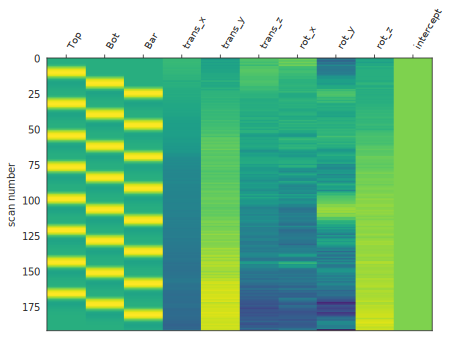
\includegraphics[keepaspectratio]{images/sub-P01_task-localizer_run-1_design.png}}
\end{itemize}

\section{Buidling regressors}\label{buidling-regressors}

\pandocbounded{\includegraphics[keepaspectratio]{images/clipboard-4230244420.png}}

Some convolution examples can be found here (Lindquist 2008)

\section{General linear model}\label{general-linear-model}

\pandocbounded{\includegraphics[keepaspectratio]{images/clipboard-3283349145.png}}

\section{Statistical inference in whole-brain
analysis}\label{statistical-inference-in-whole-brain-analysis}

\pandocbounded{\includegraphics[keepaspectratio]{images/clipboard-3973626449.png}}

How do we get from beta estimates to making statistical inference? As in
a typical regression, beta estimate divided by its standard error is a
t-statistic with a t-distribution. So to know whether an activation in
one voxel is significant is relatively straightforward.

If we had just one voxel, we would have computed the t-statistic, and
then depending on the degrees of freedom determined if it exceeds the
critical value. However, we are doing the same statistical test for MANY
voxels. SO the probability that we find a significant voxel simply by
chance increases. This is the multiple comparison problem that is
encountered anywhere in statistics. In fMRI it is particularly
prominent, because the number if singe tests is enormous. There are
several ways and philosophies for dealing with it, I won't go into
details right now. The important thing is that any voxel-wise analysis
MUST deal with this problem in some way.

\section{Two conditions}\label{two-conditions}

\pandocbounded{\includegraphics[keepaspectratio]{images/clipboard-3643081170.png}}

\section{General linear model with two
conditions}\label{general-linear-model-with-two-conditions}

\pandocbounded{\includegraphics[keepaspectratio]{images/clipboard-632029715.png}}

\section{Contrast}\label{contrast}

A linear combination of beta estimates

\pandocbounded{\includegraphics[keepaspectratio]{images/clipboard-3240858118.png}}

\section{GLM advantages}\label{glm-advantages}

\pandocbounded{\includegraphics[keepaspectratio]{images/clipboard-4292960842.png}}

\begin{itemize}
\item
  Complex experimental designs
\item
  Discounting uninteresting effects/confounds
\item
  HRF shape estimation
\end{itemize}

\section{Group analysis}\label{group-analysis}

\pandocbounded{\includegraphics[keepaspectratio]{images/clipboard-1995917989.png}}

\section{Region-of-interest (ROI)
analysis}\label{region-of-interest-roi-analysis}

\pandocbounded{\includegraphics[keepaspectratio]{images/clipboard-2858615543.png}}

Question: Does the primary visual cortex respond to flickering
checkerboards?

HCP cortical parcellation (``Glasser atlas'') (Glasser et al. 2016)

ROI analysis is a way to deal with multiple comparison problem. But it
requires an a priory and independent definition of an ROI.

There are two ways to define ROIs:

\begin{itemize}
\item
  From an anatomical scan
\item
  From an additional (separate) functional experiment
\end{itemize}

\section{Subcortical ROIs}\label{subcortical-rois}

\pandocbounded{\includegraphics[keepaspectratio]{images/next_brain_coronal.png}}

NextBrain parcellation containing 333 anatomical structures (Casamitjana
et al. 2024)

This is the state-of-the-art for anatomically-based ROI definition based
on deep learning

\section{Multivariate pattern
analysis}\label{multivariate-pattern-analysis}

\pandocbounded{\includegraphics[keepaspectratio]{images/clipboard-3955080845.png}}

Question: Is the voxel response \emph{pattern} different in condition A
and B?

Remember that an image is 4d and consists of little 3d cubes called
voxels, with the 4th dimension being time. A classical analysis is done
over time for every voxel in the brain independently. In a multivariate
analysis we first perform a univariate analysis and then look at
response patterns of multiple voxels at a time.

In this example, both coca cola and pepsi activate the same 6 voxels in
the visual cortex. But the red ones are activated more by cola then by
pepsi, and the blue ones the other way around. If you just look at the
average response over 6 voxels, you will not see a difference.

\section{Searchlight analysis}\label{searchlight-analysis}

\pandocbounded{\includegraphics[keepaspectratio]{images/clipboard-137996085.png}}

MVPA can be done for a region of interest, or for the entire brain. In
the latter case, the brain is subdivided into multiple ROIs, and the
relevant analysis is performed for each of them. This procedure is
called ``searchlight''. In this case, MCC is as relevant as it is in a
univariate analysis.

\section{First MVPA paper}\label{first-mvpa-paper}

\pandocbounded{\includegraphics[keepaspectratio]{images/clipboard-1666315153.png}}

Representation similarity analysis (Haxby et al. 2001)

\section{Machine learning}\label{machine-learning}

\pandocbounded{\includegraphics[keepaspectratio]{images/clipboard-3573273781.png}}

\pandocbounded{\includegraphics[keepaspectratio]{images/clipboard-2352405043.png}}

First MVPA papers, both appeared in 2005 (Haynes and Rees 2005; Kamitani
and Tong 2005)

\section{SVM classifier}\label{svm-classifier}

\pandocbounded{\includegraphics[keepaspectratio]{images/clipboard-845253526.png}}

Toy example for 2D feature space. Further reading in e.g.~Cohen et al.
(2017)

\section{References}\label{references}

\bookmarksetup{startatroot}

\chapter{Experimental paradigm}\label{experimental-paradigm}

In PsychoPy

\section{Runs}\label{runs}

\begin{itemize}
\item
  chunks of 5-10 minute length
\item
  one run - one start of the PsychoPy script
\end{itemize}

\section{Start screen}\label{start-screen}

\begin{itemize}
\item
  The script should start by showing a welcome message or instruction
  reminder
\item
  It should be waiting for key ``5'' (scanner ``trigger'')
\item
  This is needed to synchronize the fMRI signal acquisition with your
  paradigm
\item
  After the start screen, there should be a period of ca. 10 seconds of
  nothing happening; this is needed to discard initial artifacts
\end{itemize}

\section{Subject responses}\label{subject-responses}

Subject keys: 1, 2, 3, 4, {[}{]}, 6, 7, 8, 9

\includegraphics[width=0.5\linewidth,height=\textheight,keepaspectratio]{images/clipboard-4146499127.png}\footnote{Current
  Designs
  \url{https://www.curdes.com/mainforp/responsedevices/buttonboxes/hhsc-1x4-l.html}}

\section[BIDS plugin for PsychoPy]{\texorpdfstring{BIDS
plugin\footnote{\url{https://psychopy-bids.readthedocs.io/en/stable/}}
for
PsychoPy}{BIDS plugin for PsychoPy}}\label{bids-pluginparadigm-2-for-psychopy}

Should be installed and enabled to save events (conditions and button
presses) in a comprehensive and standardized manner

\pandocbounded{\includegraphics[keepaspectratio]{images/clipboard-4271384204.png}}

This will also make our data analysis easier

\bookmarksetup{startatroot}

\chapter{Data management}\label{data-management}

In neuroimaging

\section{General}\label{general}

\pandocbounded{\includegraphics[keepaspectratio]{images/clipboard-3125101888.png}}

\marginnote{\begin{footnotesize}

(Juavinett 2022)

\end{footnotesize}}

\section{State in 2022}\label{state-in-2022}

\pandocbounded{\includegraphics[keepaspectratio]{images/clipboard-572345686.png}}

\marginnote{\begin{footnotesize}

Image credit: (Juavinett 2022)

\end{footnotesize}}

\section{BIDS}\label{bids}

\pandocbounded{\includegraphics[keepaspectratio]{images/clipboard-4264973894.png}}

\bookmarksetup{startatroot}

\chapter{1. Psychopy}\label{psychopy}

\section{BIDS plugin for PsychoPy}\label{bids-plugin-for-psychopy}

Should be installed and enabled to save events (conditions and button
presses) in a comprehensive and standardized manner.

\pandocbounded{\includegraphics[keepaspectratio]{images/clipboard-4271384204.png}}

This will also make our data analysis easier

\marginnote{\begin{footnotesize}

\url{https://psychopy-bids.readthedocs.io/en/stable/}

\end{footnotesize}}

\section{Installation}\label{installation}

\pandocbounded{\includegraphics[keepaspectratio]{images/clipboard-3969700235.png}}

Open psychopy and press ``Get more'' on the right side. Alternatively
you can open ``plugin/pachages manager'' via ``Tools'' menue.
Psychopy-plugin should be listed among the available plugins.

On the university computers, bids plugin is available through software
center.

\bookmarksetup{startatroot}

\chapter[Experiment adjustment]{\texorpdfstring{Experiment
adjustment\footnote{valid for PsychoPy v2024.2.4}}{Experiment adjustment}}\label{experiment-adjustmentdata_management-1}

\section{Thanks to}\label{thanks-to}

\pandocbounded{\includegraphics[keepaspectratio]{images/clipboard-3961870448.png}}

Lukas currently took over the BIDS plugin development.

\section{Properties}\label{properties}

\pandocbounded{\includegraphics[keepaspectratio]{images/clipboard-3648775932.png}}

\begin{enumerate}
\def\labelenumi{\arabic{enumi}.}
\tightlist
\item
  Experiment name will correspond to the task-{[}taskname{]} properety
  in the bids dataset. It is therefore useful to have a short name
  without capital letters. This did not work on my mac, but maybe this
  is an OS issue?
\item
  Participant: switched from random code generator to 001. Since we keep
  the naming consistent with the MRI dataset, and have multiple runs, it
  is not useful to generate a new code on every run repetition
\item
  Session: changed from 001 to 1. This is just our naming convention.
  Nobody has hundreds of sessions, so we do not expect a number with
  more than two digits.
\end{enumerate}

\section{Renaming?}\label{renaming}

\subsection{File}\label{file}

\pandocbounded{\includegraphics[keepaspectratio]{images/clipboard-2219598044.png}}

\subsection{Project folder}\label{project-folder}

\pandocbounded{\includegraphics[keepaspectratio]{images/clipboard-1865608280.png}}

For the task label to work properly in the BIDS plugin, I also tried
renaming the experiment file and the folder, but this did not help.
Gambling is still spelled out with a capital ``G'' no mater what I do.
Let's stay tuned for the psychopy-bids updates.

\section{Research question}\label{research-question}

\subsection{What information do we actually need for
analysis?}\label{what-information-do-we-actually-need-for-analysis}

\pandocbounded{\includegraphics[keepaspectratio]{images/clipboard-1090987086.png}}

We should keep the research question in mind.

H1 is formulated as a one-way ANOVA with three pairwise post-hoc tests

H2 is formulated as 2x2 two-way ANOVA (at least we will simplify it to
that)

\section{Unique conditions}\label{unique-conditions}

\begin{itemize}
\item
  small win
\item
  small loss
\item
  large win
\item
  large loss
\item
  pass
\end{itemize}

\section{trials.xlsx}\label{trials.xlsx}

\pandocbounded{\includegraphics[keepaspectratio]{images/clipboard-752105472.png}}

For every trial, we should be able to identify whether it is win, loss
or pass.

For every win or loss trial, we need to know if it is a win/loss with
high stakes or with low stakes.

Note: right now we are not taking the win probability into account, but
we know that it is always low for large stakes, and large for low
stakes, so it is redundant.

\section{Side note:}\label{side-note}

\subsection{Ideal paradigm}\label{ideal-paradigm}

\begin{itemize}
\item
  Each trial type appears the same number of times
\item
  Carryover counterbalancing - each condition is equally likely to be
  preceded by each other condition (Brooks 2012)
\end{itemize}

\section{Events of interest in a
trial}\label{events-of-interest-in-a-trial}

\subsection{gamble\_trial or
gamble\_outcome?}\label{gamble_trial-or-gamble_outcome}

\pandocbounded{\includegraphics[keepaspectratio]{images/clipboard-3778340065.png}}

\subsection{Do we need key presses?}\label{do-we-need-key-presses}

\section{Adding bids events}\label{adding-bids-events}

\subsection{Scanner trigger}\label{scanner-trigger}

\pandocbounded{\includegraphics[keepaspectratio]{images/clipboard-3535149556.png}}

I am not sure if it is needed after all, but I added a bids component to
a routine that waits 10 seconds after the scanner trigger and logged its
onset.

\section{Linking to a routine \# 1}\label{linking-to-a-routine-1}

\pandocbounded{\includegraphics[keepaspectratio]{images/clipboard-2395359737.png}}

In the BIDS Event Type field you can choose between TaskEvent and
BehEvent. For now the difference does not matter much, let's choose task
event.

\section{Linking to a routine \#2}\label{linking-to-a-routine-2}

\pandocbounded{\includegraphics[keepaspectratio]{images/clipboard-674558866.png}}

Right now time 0 in our experiment is the start of the welcome screen.
We want time 0 to be the scanner trigger. Will take care of it later.

\section{Adding bids events of
interest}\label{adding-bids-events-of-interest}

\subsection{New variable
outcome\_trial}\label{new-variable-outcome_trial}

We need one variable to take 3 possible outcomes: win, loss or pass.
Therefore, I adjusted the code, adding a variable ``outcome\_trial'' for
this purpose.

\pandocbounded{\includegraphics[keepaspectratio]{images/clipboard-347898199.png}}

\section{points\_text}\label{points_text}

\pandocbounded{\includegraphics[keepaspectratio]{images/clipboard-182415314.png}}

We are creating a bids event and linking it to points\_text within the
trial (because this routine appears on every loop interation).

\section{Time stamp}\label{time-stamp}

\subsection{Time 0 - scanning onset}\label{time-0---scanning-onset}

\pandocbounded{\includegraphics[keepaspectratio]{images/clipboard-3405507570.png}}

Now we want to adjust the onset time to the scanner trigger arrival.
This is done by ticking ``Manually set values'' and putting the
difference between the onset of the current routine and the start of the
blank period.

It would have been better and more accurate to subtract the actually key
press time, but I ran out of time.

\section{Other events}\label{other-events}

\pandocbounded{\includegraphics[keepaspectratio]{images/clipboard-3834157527.png}}

Here I added two other bids events that may or may not be useful, just
in case: Trial onset and key press, including reaction times.

\section{BIDS export}\label{bids-export}

\pandocbounded{\includegraphics[keepaspectratio]{images/clipboard-1613912465.png}}

It is important to add the bidsExport routine at the end of the
experiment.

\begin{enumerate}
\def\labelenumi{\arabic{enumi}.}
\tightlist
\item
  For fMRI, the data type should be ``func''
\item
  Choose. your favourite license
\item
  Tick the box ``Add Run Nubmers'' - this should attach run numbers to
  the file names in bids format for every new run. I did not get it to
  work properly on mac (it was always run 1, overwriting the previous
  file). But supposedly it works on windows and linux.
\end{enumerate}

\section{Complete BIDS dataset}\label{complete-bids-dataset}

\subsection{Example}\label{example}

\pandocbounded{\includegraphics[keepaspectratio]{images/clipboard-806437960.png}}

This is how a complete dataset for fmri analysis should look like. You
should have functional \_bold.nii.gz files and \_events.tsv files in one
func/ folder.

\bookmarksetup{startatroot}

\chapter{2. DICOM to BIDS}\label{dicom-to-bids}

\section{Neurodesk}\label{neurodesk}

\pandocbounded{\includegraphics[keepaspectratio]{images/clipboard-3392567157.png}}

\section{MRI data formats}\label{mri-data-formats}

\begin{itemize}
\item
  DICOM - medical image format

  \begin{itemize}
  \tightlist
  \item
    .dcm .ima or nothing at all
  \end{itemize}
\item
  NIFTI - neuroimaging format we work with

  \begin{itemize}
  \tightlist
  \item
    .nii or .nii.gz
  \end{itemize}
\end{itemize}

\section{bidscoin}\label{bidscoin}

\pandocbounded{\includegraphics[keepaspectratio]{images/clipboard-404437105.png}}

\section{Shell commands}\label{shell-commands}

\pandocbounded{\includegraphics[keepaspectratio]{images/clipboard-1623492321.png}}

\begin{Shaded}
\begin{Highlighting}[]
\CommentTok{\#!/bin/bash}

\CommentTok{\# you can copypaste the following commands into the terminal window that is opened by BIDSCOINER}

\CommentTok{\# define directories}
\VariableTok{sourceFolder}\OperatorTok{=}\NormalTok{/home/jovyan/completion2/dcm}
\VariableTok{sortedFolder}\OperatorTok{=}\NormalTok{/home/jovyan/completion2/dcm\_sorted}

\CommentTok{\# check the output of the source folder}
\FunctionTok{ls} \AttributeTok{{-}l} \VariableTok{$sourceFolder}

\CommentTok{\# make the target directory with subdirectories}
\FunctionTok{mkdir} \AttributeTok{{-}p} \VariableTok{$sortedFolder}

\CommentTok{\# change to the script folder}
\BuiltInTok{cd}\NormalTok{ /home/jovyan/dicomsort/}

\CommentTok{\# run the script}
\ExtensionTok{./DICOMsort.sh} \VariableTok{$sourceFolder} \VariableTok{$sortedFolder}

\CommentTok{\# check the output of the target folder}
\FunctionTok{ls} \AttributeTok{{-}l} \VariableTok{$sortedFolder}

\CommentTok{\# run bidsmapper}
\ExtensionTok{bidsmapper} \VariableTok{$sortedFolder}\NormalTok{ /home/jovyan/completion2/bids}
\CommentTok{\# note: in the intendedFor of the fieldmap, add func/sub{-}001\_ses{-}1\_xxx\_bold.*}

\CommentTok{\# once you are happy with the mapping, run bidscoiner}
\ExtensionTok{bidscoiner} \VariableTok{$sortedFolder}\NormalTok{ /home/jovyan/completion2/bids}
\end{Highlighting}
\end{Shaded}

\section{bismapper}\label{bismapper}

\includegraphics[width=0.32\linewidth,height=\textheight,keepaspectratio]{images/clipboard-3995624064.png}

Currently, to discover the data we need to delete the content of the
``subprefix'' field and then save the bids map in the default location.
After this, run the same bidsmapper command again.

\section{Subject and session}\label{subject-and-session}

\includegraphics[width=0.5\linewidth,height=\textheight,keepaspectratio]{images/clipboard-325791456.png}

Now the bidsmapper discovered everything, but the files are not named
correctly.

Edit subject and session first.

Now we need to rename the files by clicking ``Edit'' next to every file.

\section{Editing file names:
anatomical}\label{editing-file-names-anatomical}

\includegraphics[width=0.5\linewidth,height=\textheight,keepaspectratio]{images/clipboard-1483139836.png}

anatmprage -\textgreater{} mprage in the ``acq'' filed

\section{Editing file names:
functional}\label{editing-file-names-functional}

\includegraphics[width=0.5\linewidth,height=\textheight,keepaspectratio]{images/clipboard-103624418.png}

Edit the task name and acq field

Do this for every functional file

In the intendedFor of the fieldmap, add
``func/sub-999\_ses-1\_task-completion\_acq--noise\_bold.*'' with a
wildcard. This will select all respective functional runs

Once you are happy, run bidscoiner to do the actual conversion

\section{View files}\label{view-files}

\pandocbounded{\includegraphics[keepaspectratio]{images/clipboard-3124758617.png}}

\section{MRICron}\label{mricron}

\includegraphics[width=4.64583in,height=\textheight,keepaspectratio]{images/clipboard-2244027224.png}

Now you can view the nifti files with any suitable software

\bookmarksetup{startatroot}

\chapter{3. Quality assurance}\label{quality-assurance}

\section{MRIQC}\label{mriqc}

MRIQC (Esteban et al. 2017)is a tool used for quality assurance of
bids-valid datasets. It is a bids app, meaning that it works on
bids-conform data.

\pandocbounded{\includegraphics[keepaspectratio]{images/clipboard-1260990723.png}}

\section{Running MRIQC}\label{running-mriqc}

Should take around 10 minutes

\subsection{Command line}\label{command-line}

\begin{Shaded}
\begin{Highlighting}[]
\CommentTok{\# define relevant paths}
\VariableTok{bids\_folder}\OperatorTok{=}\NormalTok{/home/jovyan/gambling/bids/}
\VariableTok{mriqc\_folder}\OperatorTok{=}\NormalTok{/home/jovyan/gambling/bids/derivatives/mriqc/}

\CommentTok{\# create mriqc directory}
\FunctionTok{mkdir} \AttributeTok{{-}p} \VariableTok{$mriqc\_folder}

\CommentTok{\# run mriqc}
\ExtensionTok{mriqc} \VariableTok{$bids\_folder} \VariableTok{$mriqc\_folder}\NormalTok{ participant }\AttributeTok{{-}{-}participant{-}label}\NormalTok{ 001}
\end{Highlighting}
\end{Shaded}

\subsection{Output}\label{output}

\includegraphics[width=4.86458in,height=\textheight,keepaspectratio]{images/clipboard-2070588200.png}

\marginnote{\begin{footnotesize}

You will see that there are html outputs for anatomical and functional
scans. They can be viewed in a browser, without actually loading the
images.

\end{footnotesize}}

\section{Anatomical}\label{anatomical}

\subsection{Noise}\label{noise}

\pandocbounded{\includegraphics[keepaspectratio]{images/clipboard-959542348.png}}

\subsection{Actual image}\label{actual-image}

\pandocbounded{\includegraphics[keepaspectratio]{images/clipboard-1251899225.png}}

\marginnote{\begin{footnotesize}

This is useful to quickly identify problems with the data. A rating
widget is also available, which is useful for large datasets.

\end{footnotesize}}

\section{Functional}\label{functional}

\pandocbounded{\includegraphics[keepaspectratio]{images/clipboard-2643957852.png}}

\pandocbounded{\includegraphics[keepaspectratio]{images/clipboard-3526589766.png}}

\pandocbounded{\includegraphics[keepaspectratio]{images/clipboard-800319650.png}}

\marginnote{\begin{footnotesize}

For functional data, in addition to spatial noise (middle) and average
image over time (right), there is a section showing temporal noise over
time. Note how the values are highest in the eyes (due to eye movements)
and in the center of the brain, due to blood pulsation.

\end{footnotesize}}

\section{Carpet plots for functional
data}\label{carpet-plots-for-functional-data}

\pandocbounded{\includegraphics[keepaspectratio]{images/clipboard-3163786376.png}}

\marginnote{\begin{footnotesize}

Carpet plot shows signal fluctuations over time (x-axis) for each voxel
(y-axis). Note how there are some patterns initially and at the end.
There should be no clear pattern during the experiment, this speaks for
good signal quality.

\end{footnotesize}}

\section*{References}\label{references-1}
\addcontentsline{toc}{section}{References}

\phantomsection\label{refs}
\begin{CSLReferences}{1}{0}
\bibitem[\citeproctext]{ref-belliveau1991}
Belliveau, J. W., D. N. Kennedy, R. C. McKinstry, B. R. Buchbinder, R.
M. Weisskoff, M. S. Cohen, J. M. Vevea, T. J. Brady, and B. R. Rosen.
1991. {``Functional Mapping of the Human Visual Cortex by Magnetic
Resonance Imaging.''} \emph{Science} 254 (5032): 716--19.
\url{https://doi.org/10.1126/science.1948051}.

\bibitem[\citeproctext]{ref-brooks2012}
Brooks, Joseph L. 2012. {``Counterbalancing for Serial Order Carryover
Effects in Experimental Condition Orders.''} \emph{Psychological
Methods} 17 (4): 600--614. \url{https://doi.org/10.1037/a0029310}.

\bibitem[\citeproctext]{ref-casamitjana2024}
Casamitjana, Adrià, Matteo Mancini, Eleanor Robinson, Loïc Peter,
Roberto Annunziata, Juri Althonayan, Shauna Crampsie, et al. 2024. {``A
Next-Generation, Histological Atlas of the Human Brain and Its
Application to Automated Brain MRI Segmentation.''}
\url{http://dx.doi.org/10.1101/2024.02.05.579016}.

\bibitem[\citeproctext]{ref-coates2024}
Coates, Adam, David Linhardt, Christian Windischberger, Anja Ischebeck,
and Natalia Zaretskaya. 2024. {``High-Resolution 7T fMRI Reveals the
Visual Zone of the Human Claustrum.''} \emph{Imaging Neuroscience} 2:
1--15. \url{https://doi.org/10.1162/imag_a_00327}.

\bibitem[\citeproctext]{ref-cohen2017}
Cohen, Jonathan D, Nathaniel Daw, Barbara Engelhardt, Uri Hasson, Kai
Li, Yael Niv, Kenneth A Norman, et al. 2017. {``Computational Approaches
to fMRI Analysis.''} \emph{Nature Neuroscience} 20 (3): 304--13.
\url{https://doi.org/10.1038/nn.4499}.

\bibitem[\citeproctext]{ref-esteban2017}
Esteban, Oscar, Daniel Birman, Marie Schaer, Oluwasanmi O. Koyejo,
Russell A. Poldrack, and Krzysztof J. Gorgolewski. 2017. {``MRIQC:
Advancing the Automatic Prediction of Image Quality in MRI from Unseen
Sites.''} Edited by Boris C Bernhardt. \emph{PLOS ONE} 12 (9): e0184661.
\url{https://doi.org/10.1371/journal.pone.0184661}.

\bibitem[\citeproctext]{ref-esteban2018}
Esteban, Oscar, Christopher J. Markiewicz, Ross W. Blair, Craig A.
Moodie, A. Ilkay Isik, Asier Erramuzpe, James D. Kent, et al. 2018.
{``fMRIPrep: A Robust Preprocessing Pipeline for Functional MRI.''}
\emph{Nature Methods} 16 (1): 111--16.
\url{https://doi.org/10.1038/s41592-018-0235-4}.

\bibitem[\citeproctext]{ref-glasser2016}
Glasser, Matthew F., Timothy S. Coalson, Emma C. Robinson, Carl D.
Hacker, John Harwell, Essa Yacoub, Kamil Ugurbil, et al. 2016. {``A
Multi-Modal Parcellation of Human Cerebral Cortex.''} \emph{Nature} 536
(7615): 171--78. \url{https://doi.org/10.1038/nature18933}.

\bibitem[\citeproctext]{ref-haxby2001}
Haxby, J V, M I Gobbini, M L Furey, A Ishai, J L Schouten, and P
Pietrini. 2001. {``Distributed and Overlapping Representations of Faces
and Objects in Ventral Temporal Cortex.''} \emph{Science (New York,
N.Y.)} 293 (5539): 2425--30.
\url{https://doi.org/10.1126/science.1063736}.

\bibitem[\citeproctext]{ref-haynes2005}
Haynes, John-Dylan, and Geraint Rees. 2005. {``Predicting the
Orientation of Invisible Stimuli from Activity in Human Primary Visual
Cortex.''} \emph{Nature Neuroscience} 8 (5): 686--91.
\url{https://doi.org/10.1038/nn1445}.

\bibitem[\citeproctext]{ref-interpre2009}
{``Interpreting the BOLD Response.''} 2009. In, 400--424. Cambridge
University Press. \url{https://doi.org/10.1017/cbo9780511605505.020}.

\bibitem[\citeproctext]{ref-juavinett2022}
Juavinett, Ashley L. 2022. {``The Next Generation of Neuroscientists
Needs to Learn How to Code, and We Need New Ways to Teach Them.''}
\emph{Neuron} 110 (4): 576--78.
\url{https://doi.org/10.1016/j.neuron.2021.12.001}.

\bibitem[\citeproctext]{ref-kamitani2005}
Kamitani, Yukiyasu, and Frank Tong. 2005. {``Decoding the Visual and
Subjective Contents of the Human Brain.''} \emph{Nature Neuroscience} 8
(5): 679--85. \url{https://doi.org/10.1038/nn1444}.

\bibitem[\citeproctext]{ref-lindquist2008}
Lindquist, Martin A. 2008. {``The Statistical Analysis of fMRI Data.''}
\emph{Statistical Science} 23 (4).
\url{https://doi.org/10.1214/09-sts282}.

\bibitem[\citeproctext]{ref-logothetis2001a}
Logothetis, Nikos K., Jon Pauls, Mark Augath, Torsten Trinath, and Axel
Oeltermann. 2001. {``Neurophysiological Investigation of the Basis of
the fMRI Signal.''} \emph{Nature} 412 (6843): 150--57.
\url{https://doi.org/10.1038/35084005}.

\bibitem[\citeproctext]{ref-sandrone2013}
Sandrone, Stefano, Marco Bacigaluppi, Marco R. Galloni, Stefano F.
Cappa, Andrea Moro, Marco Catani, Massimo Filippi, Martin M. Monti,
Daniela Perani, and Gianvito Martino. 2013. {``Weighing Brain Activity
with the Balance: Angelo Mosso{'}s Original Manuscripts Come to
Light.''} \emph{Brain} 137 (2): 621--33.
\url{https://doi.org/10.1093/brain/awt091}.

\bibitem[\citeproctext]{ref-zaretskaya2018}
Zaretskaya, Natalia, Bruce Fischl, Martin Reuter, Ville Renvall, and
Jonathan R Polimeni. 2018. {``Advantages of Cortical Surface
Reconstruction Using Submillimeter 7 t MEMPRAGE.''} \emph{NeuroImage}
165 (January): 11--26.
\url{https://doi.org/10.1016/j.neuroimage.2017.09.060}.

\end{CSLReferences}




\end{document}
